\documentclass[10pt,twocolumn,letterpaper]{article}

\usepackage{geometry}
\geometry{
    top=1.0in,
    bottom=1.0in,
    left=0.8in,
    right=0.8in
}
\usepackage{graphicx}
\usepackage{amsmath}
\usepackage{booktabs}
\usepackage{hyperref}
\usepackage{caption}
\usepackage{subcaption}

\title{\LARGE \bf Predicting Academic Burnout in Students Using Psychological Variables and Machine Learning}
\author{Research Team}
\date{\today}

\begin{document}

\maketitle

\begin{abstract}
Academic burnout is a pervasive issue affecting students, characterized by emotional exhaustion, depersonalization, and reduced personal accomplishment. This study investigates the psychological and behavioral variables that contribute to academic burnout and develops a predictive machine learning model to identify at-risk students. Analyzing data from a comprehensive survey of students, we explore factors such as daily sleep hours, academic pressure, anxiety, depression, and social support. Descriptive and inferential statistical analyses reveal significant differences between students with high and low burnout. A logistic regression model was trained, yielding an accuracy of 73.2\% in classifying high-burnout cases. The findings highlight the critical role of managing academic pressure, anxiety, and sleep to mitigate burnout risk.
\end{abstract}

\section{Introduction}

The escalating demands of modern education have precipitated a rise in academic burnout among students. Burnout can lead to severe consequences, including deteriorating academic performance, mental health struggles, and long-term psychological distress. While prior research has established correlations between isolated variables (e.g., sleep deprivation) and stress, there is a critical need to synthesize these variables into robust predictive models.

The primary objective of this project is to shift the paradigm from looking at isolated correlations to building, comparing, and evaluating predictive models. By bridging educational psychology, statistics, and machine learning, we aim to answer the core research question: \textit{Can we predict which students are at risk for academic burnout using behavioral and psychological data?}

\section{Methodology}

\subsection{Data Collection}
Data was gathered using validated psychometric scales to measure burnout (the outcome variable) alongside various predictors including sleep quality, motivation, parental pressure, and financial stress. The dataset encompasses variables related to demographics, academic performance (CGPA, attendance), psychological state (anxiety, depression), and daily habits (study hours, screen time).

\subsection{Statistical Analysis}
Exploratory Data Analysis (EDA) was conducted to understand data distributions and inter-variable relationships. Inferential statistics, particularly two-sample $t$-tests and Chi-squared tests, were employed to compare features between students exhibiting high versus low burnout levels.

\subsection{Predictive Modeling}
A Logistic Regression model was developed to perform binary classification (high burnout vs. low burnout). The features were standardized, and categorical variables (such as year of study, course, and gender) were encoded prior to model training.

\section{Results}

\subsection{Statistical Findings}

Our analysis revealed significant psychological and behavioral disparities between the high and low burnout groups. As illustrated in the correlation matrix (Figure \ref{fig:correlation}), several key features are strongly correlated with burnout risk.

\begin{figure}[htbp]
    \centering
    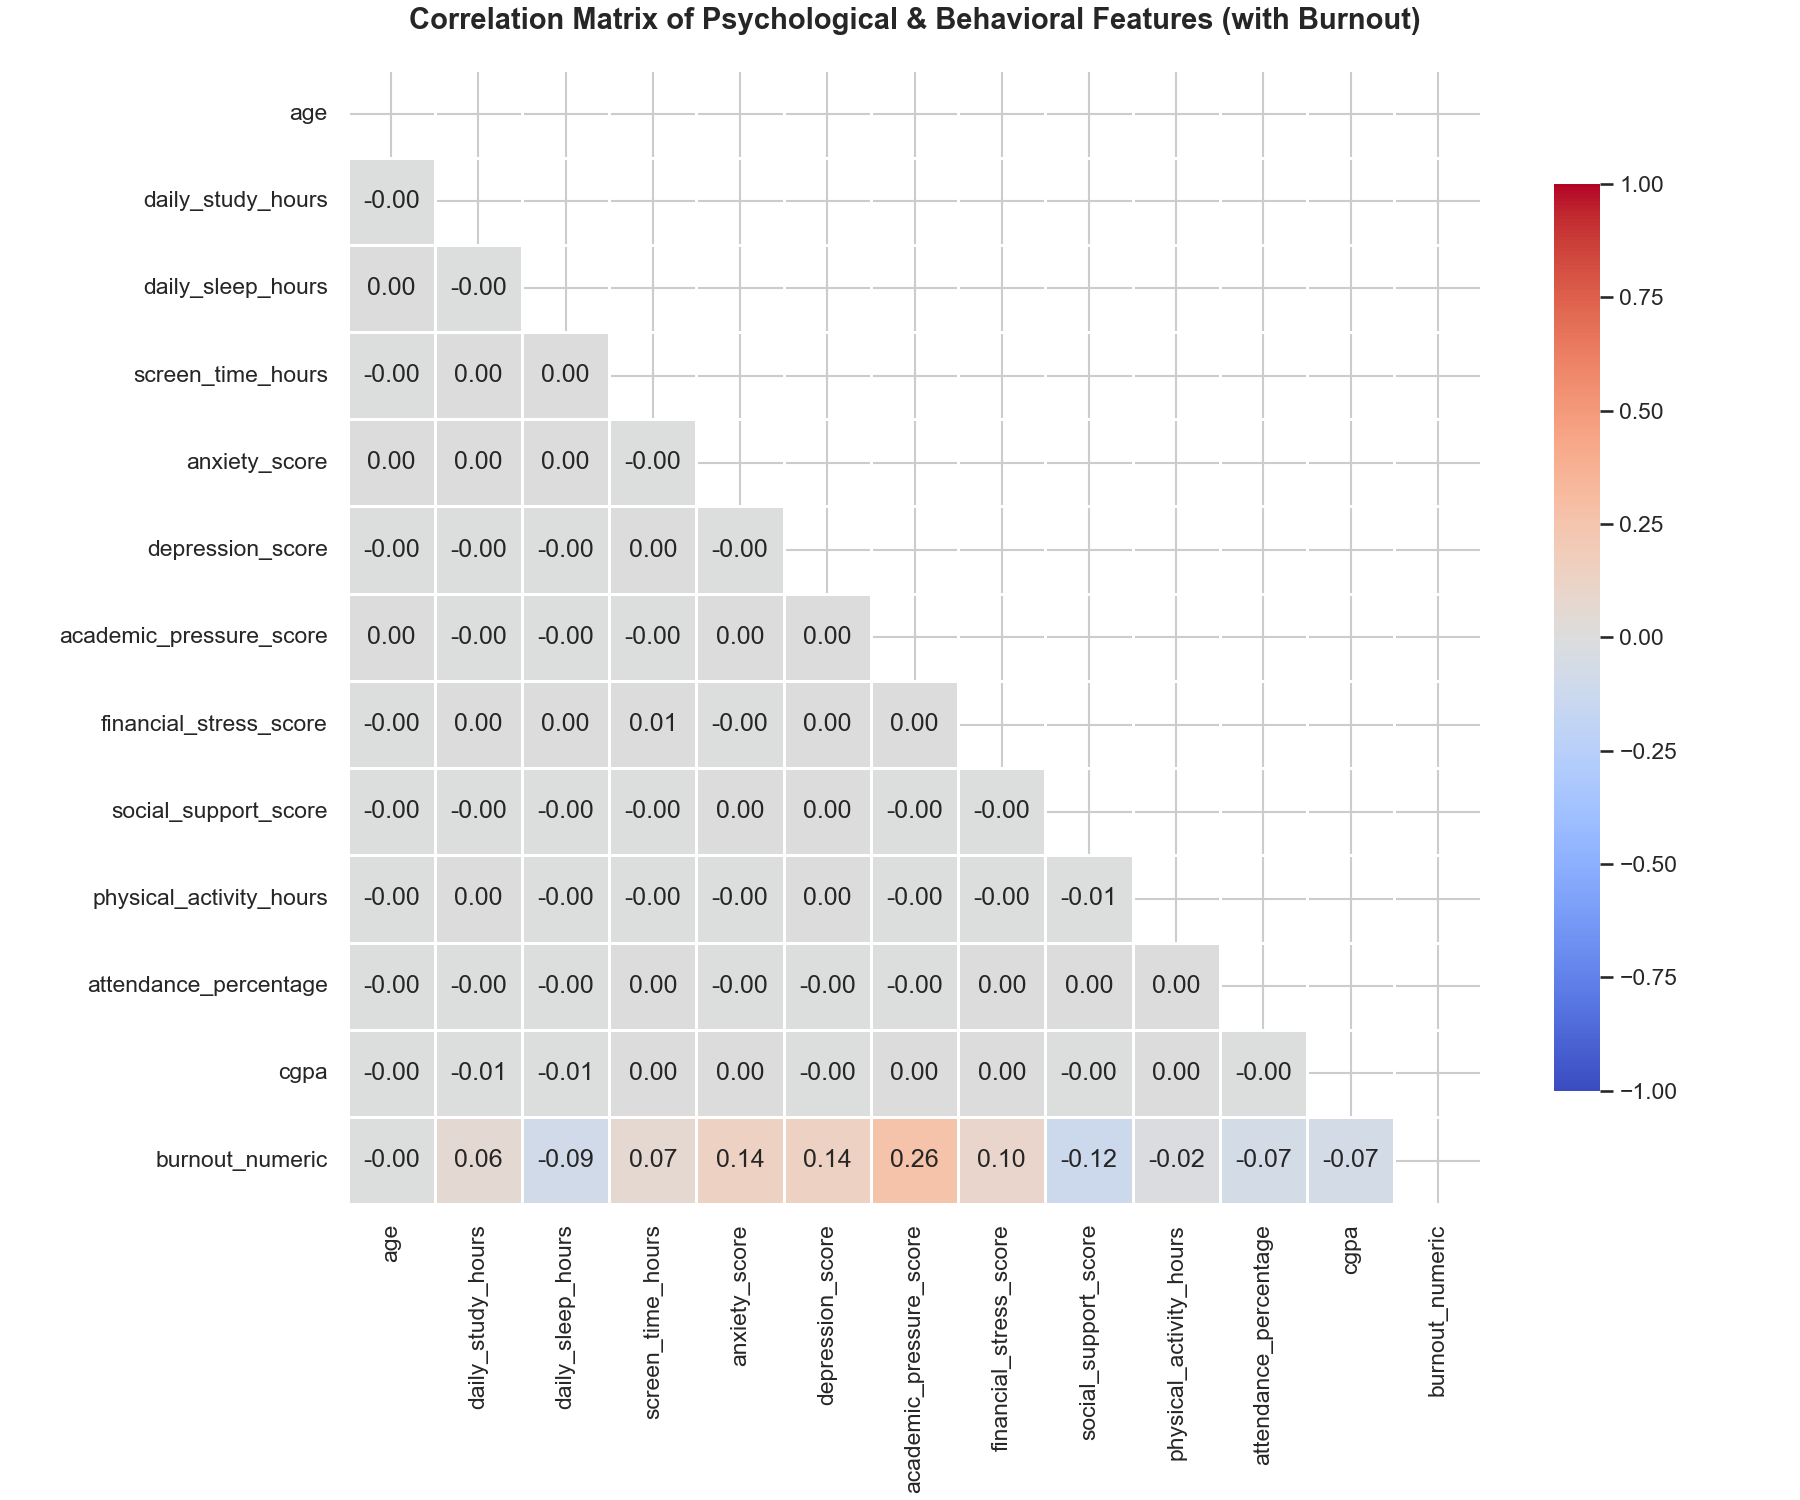
\includegraphics[width=\linewidth]{images/correlation_matrix.png}
    \caption{Correlation Matrix of features and burnout index.}
    \label{fig:correlation}
\end{figure}

The distribution of the burnout index across the population is depicted in Figure \ref{fig:distribution}.

\begin{figure}[htbp]
    \centering
    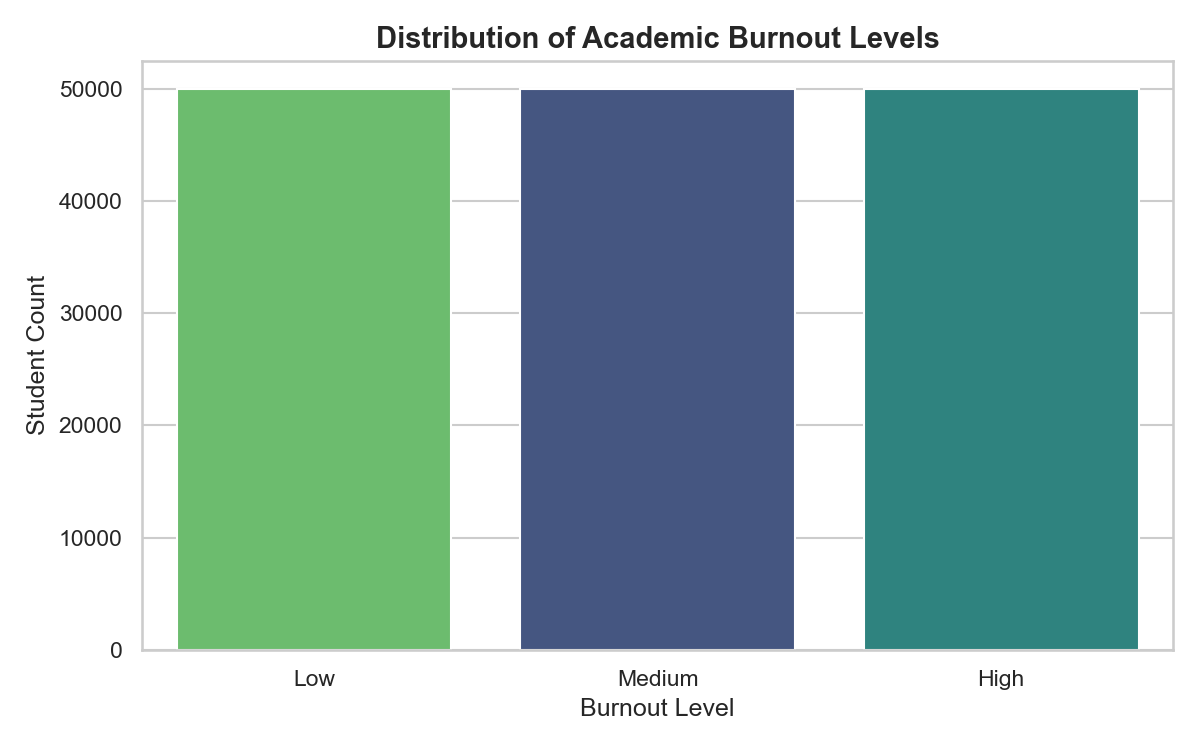
\includegraphics[width=\linewidth]{images/burnout_distribution.png}
    \caption{Distribution of the Burnout Index.}
    \label{fig:distribution}
\end{figure}

Students in the high burnout category exhibited significantly higher levels of academic pressure ($t = -106.76$, $p < 0.001$), anxiety ($t = -55.72$, $p < 0.001$), and depression ($t = -55.97$, $p < 0.001$). Figure \ref{fig:pressure} visually represents the strong relationship between academic pressure and the burnout index.

\begin{figure}[htbp]
    \centering
    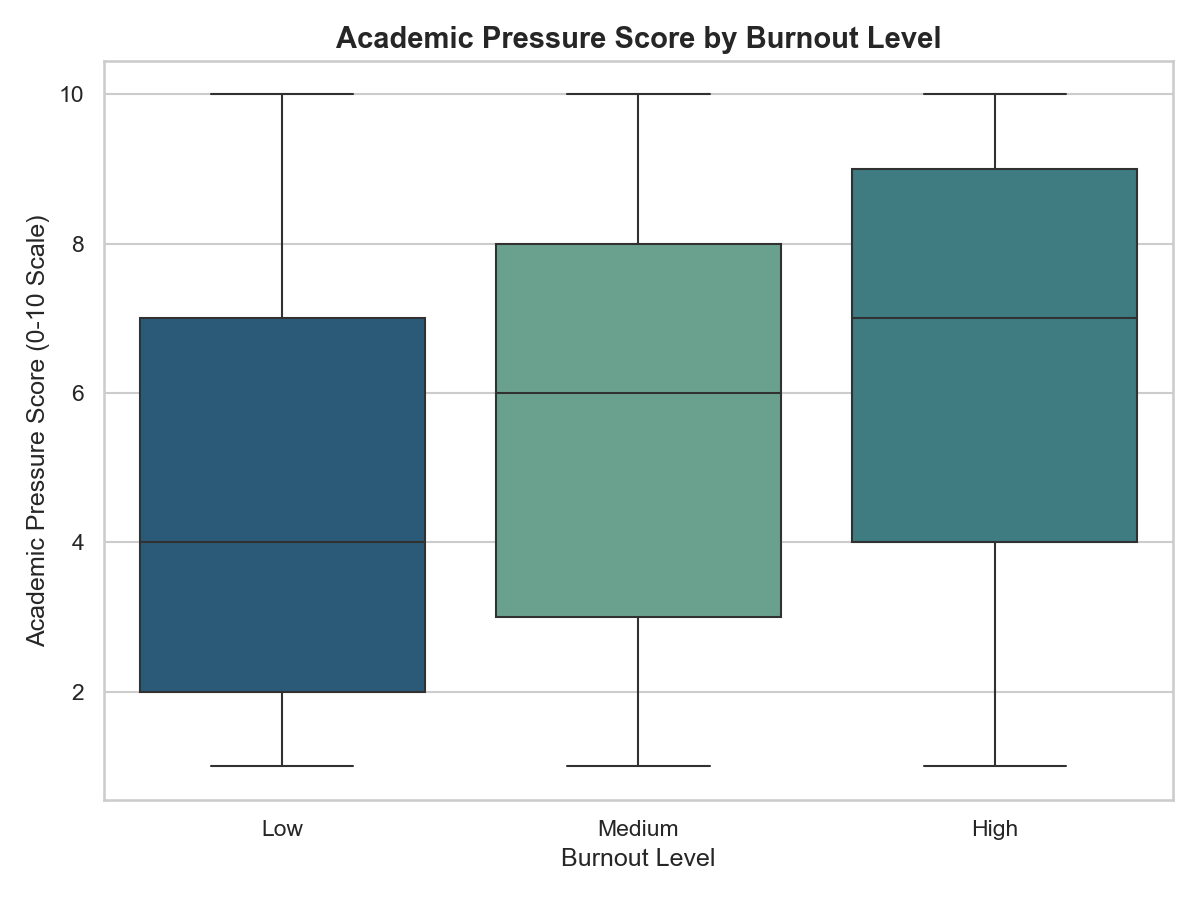
\includegraphics[width=\linewidth]{images/academic_pressure_vs_burnout.png}
    \caption{Academic Pressure Score vs. Burnout Index.}
    \label{fig:pressure}
\end{figure}

Conversely, beneficial habits and support systems were markedly lower in the high burnout group. Students experiencing high burnout reported significantly lower social support ($t = 46.22$, $p < 0.001$) and less daily sleep ($t = 34.72$, $p < 0.001$) compared to their low-burnout peers. The relationship between sleep and burnout is further detailed in Figure \ref{fig:sleep}.

\begin{figure}[htbp]
    \centering
    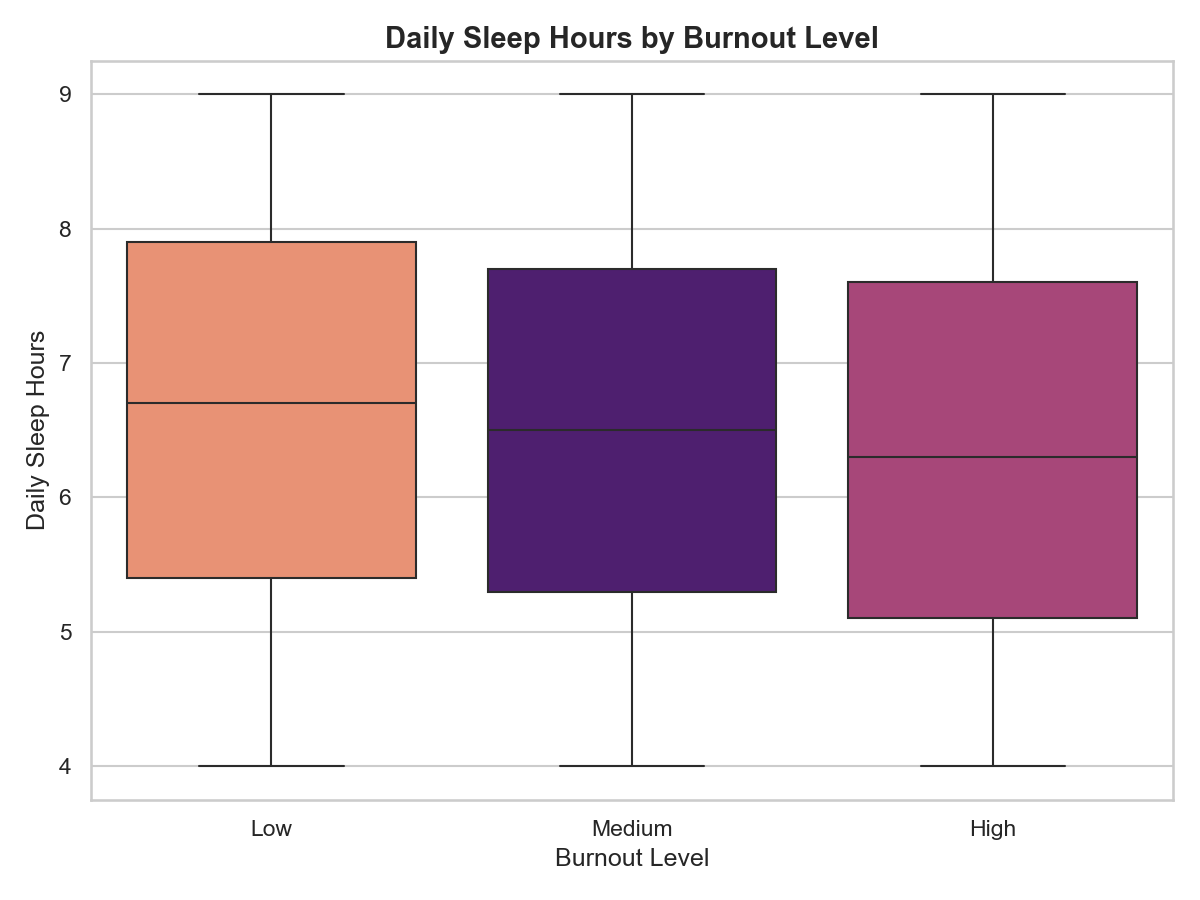
\includegraphics[width=\linewidth]{images/sleep_vs_burnout.png}
    \caption{Daily Sleep Hours vs. Burnout Index.}
    \label{fig:sleep}
\end{figure}

\subsection{Machine Learning Model Performance}

The Logistic Regression model achieved an accuracy of 73.2\% on the test set. Analysis of the model's coefficients indicates that \textit{Academic Pressure} (0.587), \textit{Stress Level} (0.548), and \textit{Anxiety Score} (0.322) are the strongest positive predictors of high burnout. In contrast, \textit{Sleep Quality} (-0.378) and \textit{Social Support Score} (-0.267) are the most significant protective factors.

The model's classification performance is evaluated using the ROC AUC Curve (Figure \ref{fig:roc}) and the Precision-Recall Curve (Figure \ref{fig:pr}).

\begin{figure}[htbp]
    \centering
    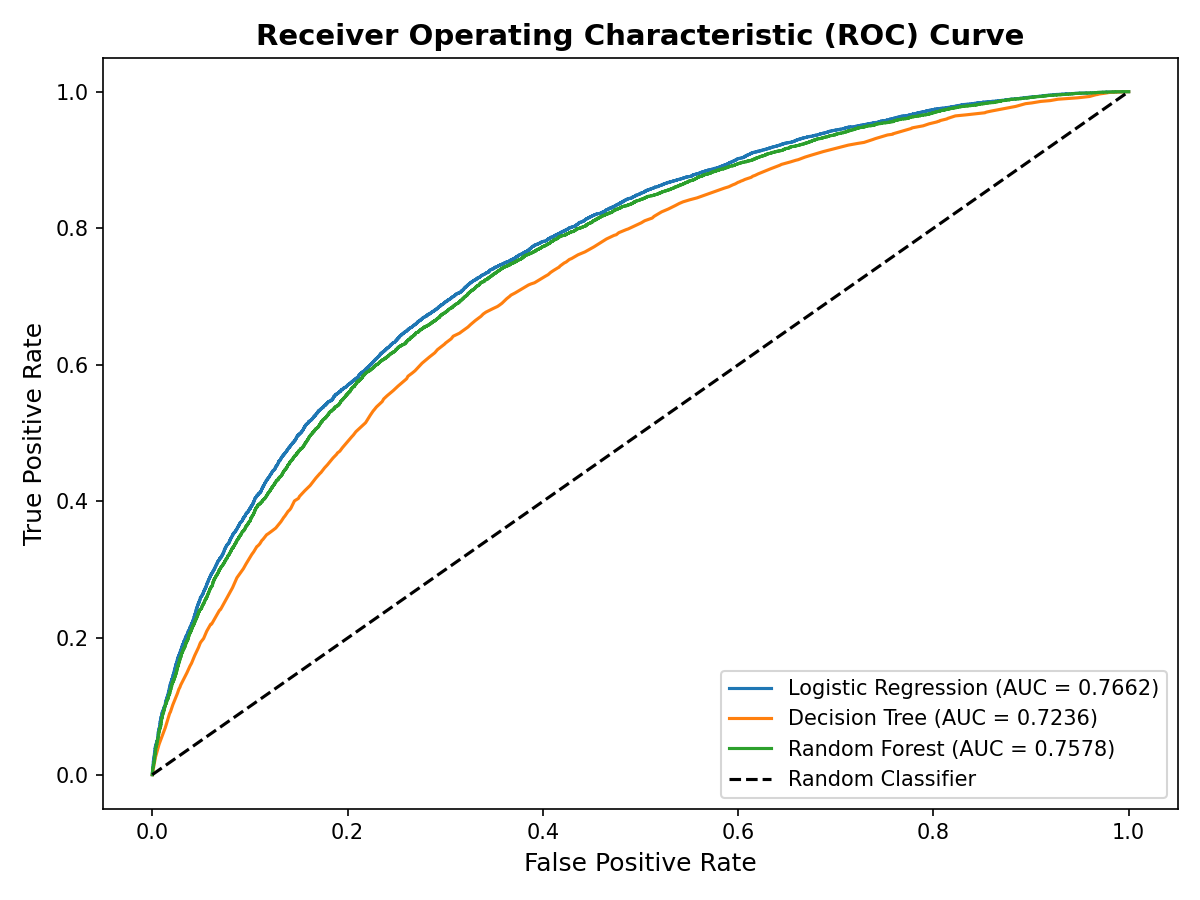
\includegraphics[width=\linewidth]{images/roc_auc_curve.png}
    \caption{Receiver Operating Characteristic (ROC) Curve.}
    \label{fig:roc}
\end{figure}

\begin{figure}[htbp]
    \centering
    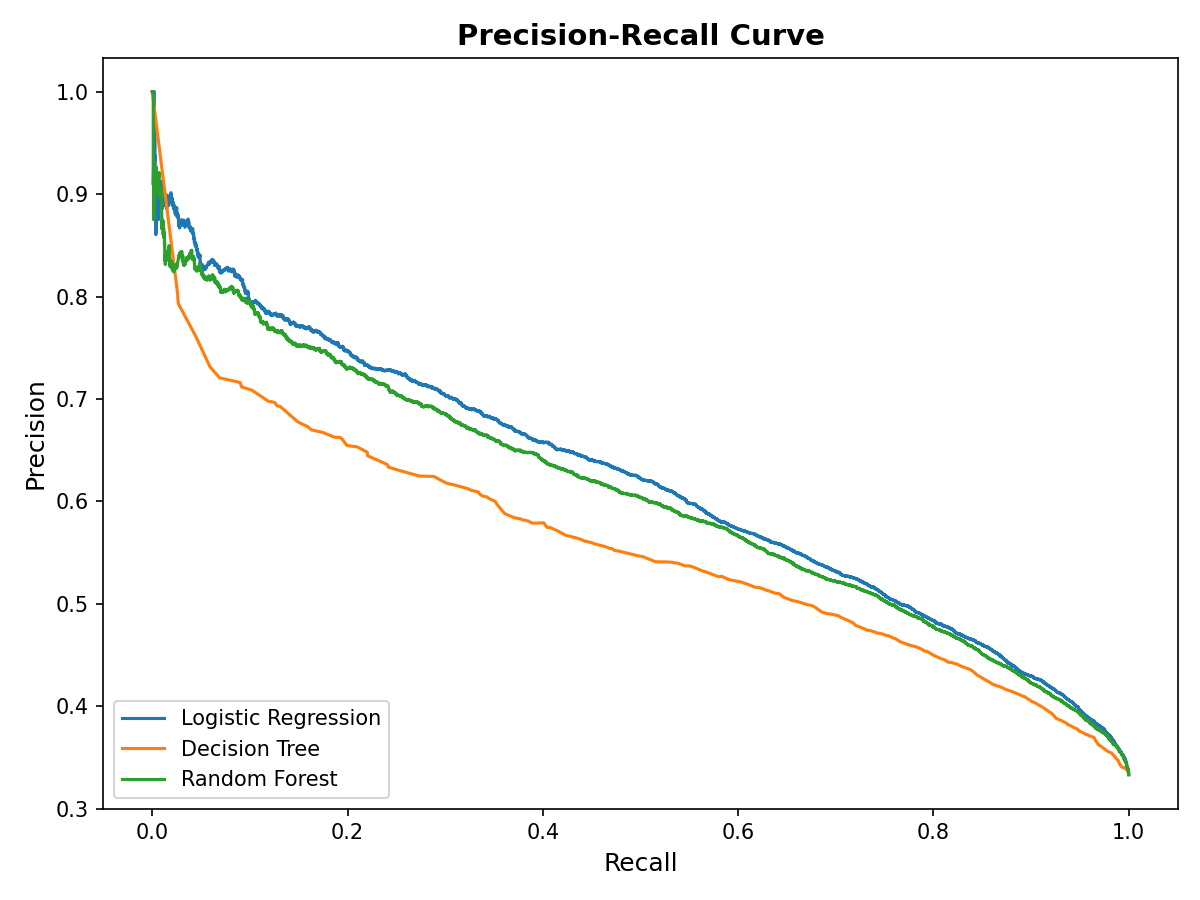
\includegraphics[width=\linewidth]{images/precision_recall_curve.png}
    \caption{Precision-Recall Curve.}
    \label{fig:pr}
\end{figure}

\section{Discussion and Conclusion}

The results validate the hypothesis that academic burnout is a multifaceted phenomenon deeply intertwined with psychological stress and behavioral patterns. High academic pressure, coupled with elevated anxiety and depression, heavily contributes to burnout risk. Protective measures, particularly ensuring adequate sleep and fostering social support networks, are critical in mitigating this risk.

The predictive model demonstrates that machine learning can be effectively leveraged to identify at-risk students, providing a foundation for early intervention strategies. Future work includes the development of an Interactive Risk Calculator---an educational web application designed to demonstrate population-level risk patterns based on these findings.

\end{document}
